\appendix
\section{Questionnaire: Evaluation of Models by Domain Experts}
\label{appendix:questionnaire}

To ensure the practical relevance and effectiveness of the proposed models for vulnerability classification and remediation, an expert evaluation was conducted. The aim was to gather insights regarding the clarity, usability, and alignment of the models with real-world practices. Domain experts were invited to assess the following components:

\begin{itemize}
    \item \textbf{Multi-Dimensional Classification Model:} 
    This model integrates \ac{CVSS} and \ac{EPSS} scores to provide a comprehensive severity rating for software vulnerabilities. Experts evaluated the clarity and practicality of merging these scores and the appropriateness of the weighting approach.

    \item \textbf{Remediation Model (\ac{SSVC}-inspired):}
    A decision-making framework providing tailored remediation recommendations based on exploit likelihood, patch availability, and asset criticality. The experts assessed whether the proposed decision flows align with current industry practices.

    \item \textbf{Rank-Ordering Mechanism:}
    A prioritization approach that highlights critical and data-incomplete vulnerabilities to streamline remediation efforts. Experts provided feedback on whether this prioritization reflects typical approaches used in practice.
\end{itemize}

The valuable feedback obtained from this evaluation directly influenced the refinement of the models, ensuring their applicability in real-world environments. It will also guide upcoming research in this area.

\textit{Note: The appendix contains the original questionnaire as an embedded PDF with separate pagination. The main thesis continues after the embedded document.}

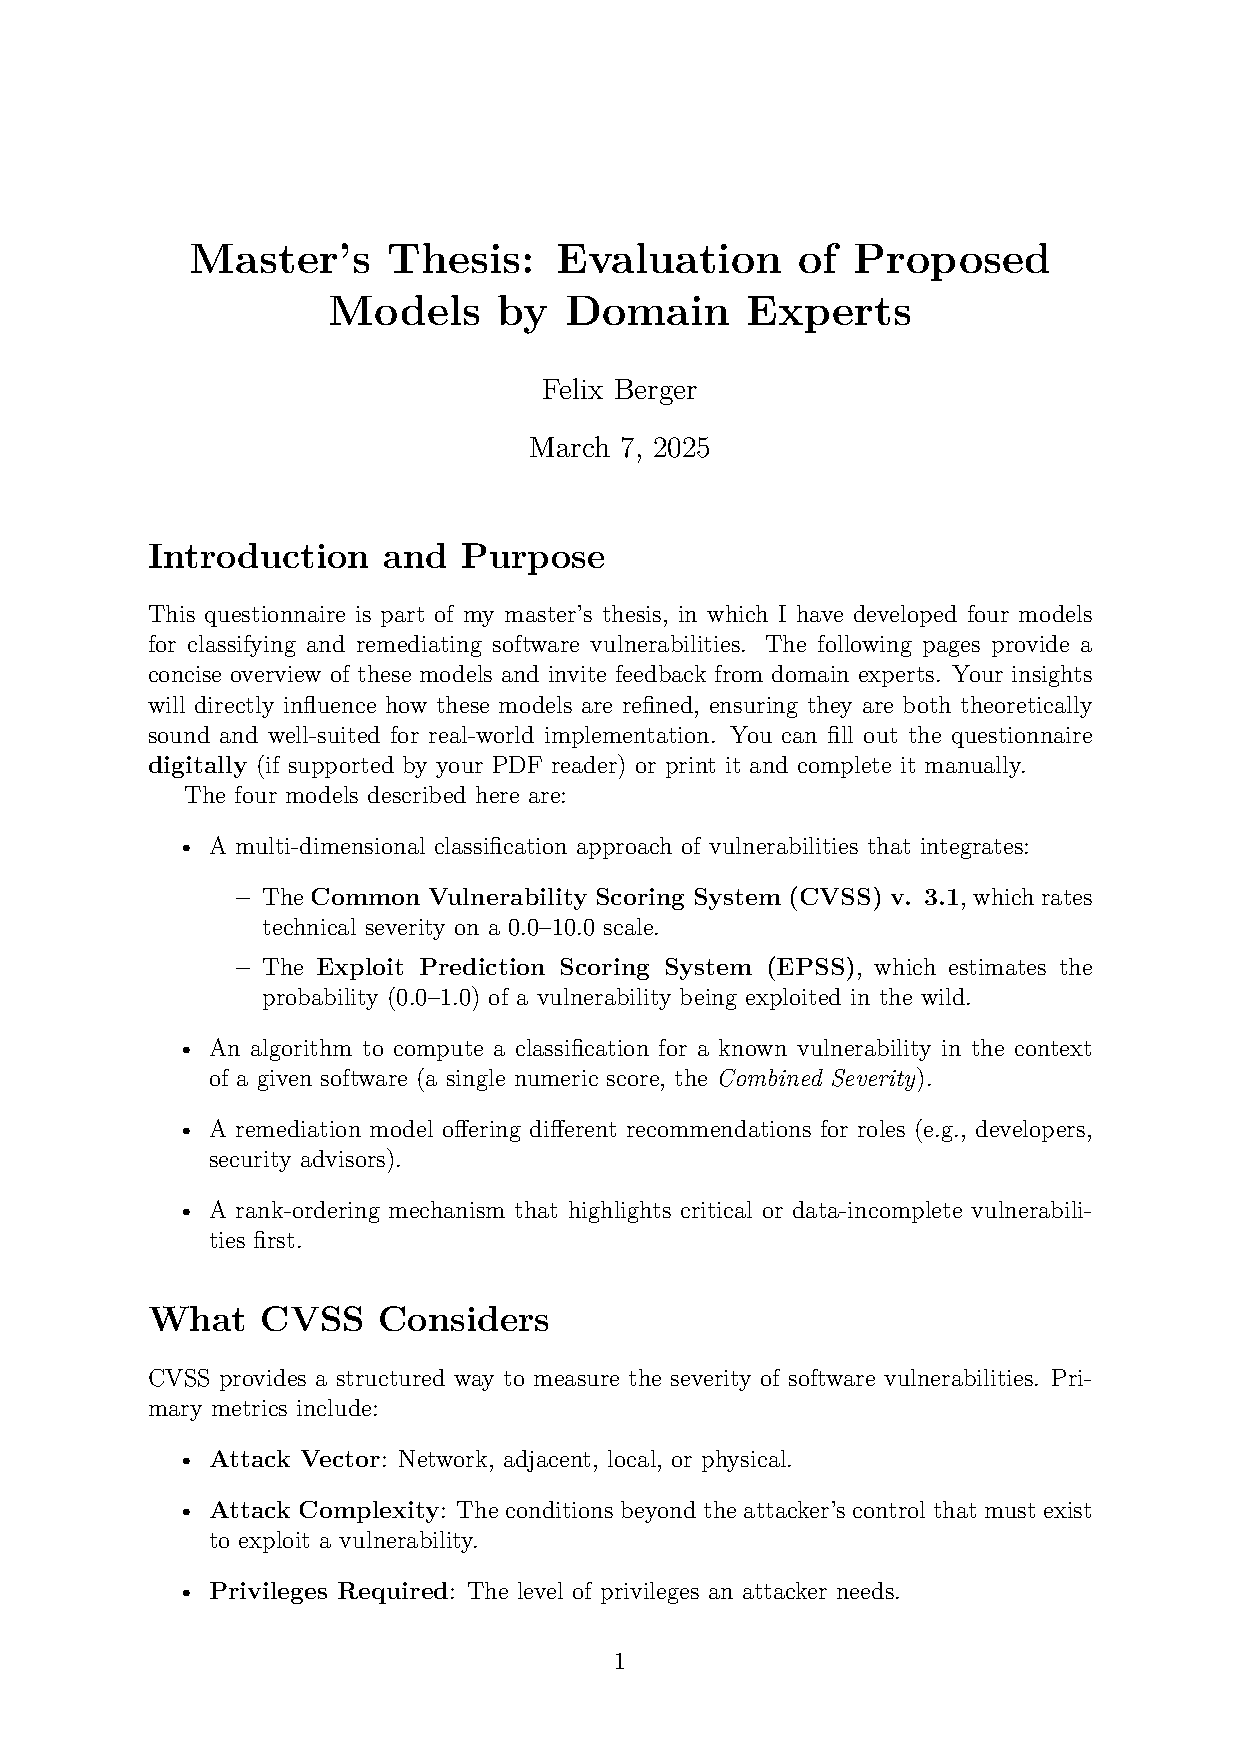
\includepdf[pages=-]{resources/Master_Thesis_Questionnaire.pdf}
